\documentclass[11pt,a4paper]{article}
\usepackage[utf8]{inputenc}
\usepackage[vietnamese]{babel}
\usepackage{amsmath,amssymb}
\usepackage[version=4]{mhchem}
\usepackage{geometry}
\geometry{top=1.5cm,bottom=1.2cm,left=1.4cm,right=1.4cm,headheight=28pt,headsep=12pt,footskip=18pt}
\usepackage{graphicx}
\usepackage{xcolor}
\usepackage{tabularx}
\usepackage{array}
\usepackage{colortbl}
\usepackage{tikz}
\usepackage{chemfig}
\usepackage{fancyhdr}
\usepackage{enumitem}
\usepackage{multido}
\usepackage{tcolorbox}

\definecolor{hfRed}{HTML}{D32F2F}
\definecolor{hfGreen}{HTML}{8BC390}
\definecolor{mainGreen}{HTML}{2E7D32}
\definecolor{solBlue}{HTML}{1565C0}
\definecolor{tableGreen}{HTML}{E8F5E9}

\usepackage{ex_test}

\pagestyle{fancy}
\fancyhf{}
\renewcommand{\headrulewidth}{0.75pt}
\renewcommand{\headrule}{\hbox to\headwidth{\color{hfGreen}\leaders\hrule height \headrulewidth\hfill}}
\renewcommand{\footrulewidth}{0.75pt}
\renewcommand{\footrule}{\hbox to\headwidth{\color{hfGreen}\leaders\hrule height \footrulewidth\hfill}}

\fancyhead[L]{\small\itshape\color{hfRed}Tài liệu lưu hành nội bộ}
\fancyhead[R]{\small\color{hfRed}Thầy \textbf{TRẦN VĂN THẠNH} - 0777.470.803}

\fancyfoot[L]{\footnotesize\itshape\color{hfRed}CS1: 6/15 Nguyễn Hoàng, P. Kim Long, TP Huế \quad|\quad CS2: 24 Đặng Thái Thân, TP Huế}
\fancyfoot[R]{\small\textbf{\color{hfRed}Trang \thepage}}

\setlength{\parindent}{0pt}
\setlength{\parskip}{2pt}

\begin{document}

\begin{minipage}[t]{0.48\textwidth}
\textbf{SỞ GD \& ĐT THÀNH PHỐ HUẾ}\\
\textbf{TRƯỜNG THPT GIA HỘI}\\
\textit{ĐỀ CHÍNH THỨC}\\
\textit{(Đề thi có 03 trang)}
\end{minipage}
\hfill
\begin{minipage}[t]{0.48\textwidth}
\raggedleft
\textbf{\color{hfRed}KIỂM TRA GIỮA KÌ II}\\
\textbf{NĂM HỌC 2025 -- 2026}\\
\textbf{MÔN: HOÁ HỌC LỚP 11}\\
\textit{Thời gian làm bài: 45 phút (không kể thời gian phát đề)}\\
\textbf{MÃ ĐỀ THI: 2608}
\end{minipage}

\vspace{4pt}
\noindent
\textit{Họ tên thí sinh:} \dotfill \textit{Lớp:} \dotfill \textit{Số báo danh:} \dotfill

\vspace{3pt}
\noindent
\textit{\footnotesize Cho nguyên tử khối của các nguyên tố: $\ce{H}=1; \ce{C}=12; \ce{O}=16; \ce{Cl}=35{,}5; \ce{Ag}=108; \ce{Br}=80; \ce{N}=14$.}

\vspace{3pt}
\hrule color{hfGreen} height 0.5pt

\vspace{4pt}
\begin{center}
\textbf{\color{hfRed}\large (BẢN GIÁO VIÊN -- CÓ LỜI GIẢI CHI TIẾT)}
\end{center}

\vspace{2pt}
\begin{center}
{\color{hfRed}\textbf{\large BẢNG ĐÁP ÁN RÚT GỌN (DÀNH CHO GIÁO VIÊN)}}
\end{center}

\vspace{2pt}
\noindent
\textbf{\color{mainGreen}1. Phần I: Trắc nghiệm nhiều lựa chọn (3,0 điểm - mỗi câu đúng 0,25 điểm)}
\begin{center}
\renewcommand{\arraystretch}{1.2}
\begin{tabular}{|c|c|c|c|c|c|c|c|c|c|c|c|c|}
\hline
\rowcolor{tableGreen}
\textbf{Câu} & \textbf{1} & \textbf{2} & \textbf{3} & \textbf{4} & \textbf{5} & \textbf{6} & \textbf{7} & \textbf{8} & \textbf{9} & \textbf{10} & \textbf{11} & \textbf{12} \\
\hline
\textbf{Đ/A} & \textbf{\color{hfRed}A} & \textbf{\color{hfRed}B} & \textbf{\color{hfRed}C} & \textbf{\color{hfRed}D} & \textbf{\color{hfRed}C} & \textbf{\color{hfRed}B} & \textbf{\color{hfRed}D} & \textbf{\color{hfRed}B} & \textbf{\color{hfRed}A} & \textbf{\color{hfRed}C} & \textbf{\color{hfRed}A} & \textbf{\color{hfRed}D} \\
\hline
\end{tabular}
\end{center}

\vspace{2pt}
\noindent
\textbf{\color{mainGreen}2. Phần II: Trắc nghiệm Đúng / Sai (2,0 điểm - mỗi câu 1,0 điểm)}
\begin{center}
\renewcommand{\arraystretch}{1.2}
\begin{tabular}{|c|l|c|c|c|c|}
\hline
\rowcolor{tableGreen}
\textbf{Câu} & \textbf{Nội dung câu hỏi} & \textbf{Ý a} & \textbf{Ý b} & \textbf{Ý c} & \textbf{Ý d} \\
\hline
\textbf{Câu 1} & Thí nghiệm điều chế và thử tính chất ethylene & \textbf{\color{hfRed}ĐÚNG} & \textbf{SAI} & \textbf{\color{hfRed}ĐÚNG} & \textbf{\color{hfRed}ĐÚNG} \\
\hline
\textbf{Câu 2} & Benzene, toluene và styrene (Arene) & \textbf{SAI} & \textbf{SAI} & \textbf{\color{hfRed}ĐÚNG} & \textbf{SAI} \\
\hline
\end{tabular}
\end{center}

\vspace{2pt}
\noindent
\textbf{\color{mainGreen}3. Phần III: Trả lời ngắn (2,0 điểm - mỗi câu đúng 0,5 điểm)}
\begin{center}
\renewcommand{\arraystretch}{1.2}
\begin{tabular}{|c|c|c|c|c|}
\hline
\rowcolor{tableGreen}
\textbf{Câu} & \textbf{Câu 1} & \textbf{Câu 2} & \textbf{Câu 3} & \textbf{Câu 4} \\
\hline
\textbf{Đáp án} & \textbf{\color{hfRed}3} & \textbf{\color{hfRed}90,6\%} & \textbf{\color{hfRed}4} & \textbf{\color{hfRed}4958} \\
\hline
\end{tabular}
\end{center}

\vspace{2pt}
\noindent
\textbf{\color{mainGreen}4. Tóm tắt đáp số Phần Tự luận (3,0 điểm)}
\begin{center}
\renewcommand{\arraystretch}{1.2}
\begin{tabular}{|c|c|p{11.5cm}|}
\hline
\rowcolor{tableGreen}
\textbf{Câu} & \textbf{Điểm} & \textbf{Đáp số cốt lõi} \\
\hline
\textbf{Câu 1} & 1,0 đ & $n_{\ce{C3H8}} = \frac{12000}{44}\text{ mol} \implies V = \frac{12000}{44} \times 24{,}79 \approx \mathbf{6760{,}91\text{ Lít}}$ (đkc $25^\circ\text{C}, 1\text{ bar}$). \\
\hline
\textbf{Câu 2} & 1,0 đ & (1) $\ce{CH#CH + H2 ->[Pd/PbCO3, t^o] CH2=CH2}$ \quad (2) $n\,\ce{CH2=CH2 ->[t^o, p, xt] (-CH2-CH2-)_n}$ \\
\hline
\textbf{Câu 3} & 1,0 đ & $n_{\text{toluene}} = \frac{552{,}0}{92} = 6{,}0\text{ mol} \implies n_{\text{TNT (TT)}} = 6{,}0 \times 60\% = 3{,}6\text{ mol} \implies m_{\text{TNT}} = 3{,}6 \times 227 = \mathbf{817{,}2\text{ g}}$. \\
\hline
\end{tabular}
\end{center}

\vspace{4pt}
\hrule color{hfGreen} height 0.5pt

\vspace{4pt}
\noindent
{\color{mainGreen}\textbf{\large I. TRẮC NGHIỆM NHIỀU LỰA CHỌN: (12 câu -- 3,0 điểm)}}\\
\textit{\small (Học sinh chọn đáp án đúng nhất. Mỗi câu trả lời đúng được 0,25 điểm)}
\vspace{2pt}

\begin{ex}
Phản ứng thế giữa 2,3-dimethylbutane với $\ce{Cl2}$ (tỉ lệ mol 1:1) cho mấy sản phẩm thế?
\choice
{\True 2.}
{5.}
{3.}
{4.}

\loigiai{
Công thức cấu tạo của 2,3-dimethylbutane: $\ce{CH3-CH(CH3)-CH(CH3)-CH3}$.\\
Phân tử có tính đối xứng cao:\\
- 4 nhóm $\ce{-CH3}$ ở hai đầu tương đương nhau (12 nguyên tử $\ce{H}$) $\implies$ thế 1 nguyên tử $\ce{Cl}$ vào nhóm $\ce{-CH3}$ cho 1 sản phẩm: 1-chloro-2,3-dimethylbutane.\\
- 2 nhóm $\ce{-CH<}$ tương đương nhau (2 nguyên tử $\ce{H}$) $\implies$ thế 1 nguyên tử $\ce{Cl}$ vào nhóm $\ce{-CH<}$ cho 1 sản phẩm: 2-chloro-2,3-dimethylbutane.\\
Vậy số sản phẩm thế monoclo (cấu tạo) thu được là 2.\\
\textbf{Chọn A.}
}
\end{ex}
\begin{ex}
Cho 5 chất: $\ce{CH3CH2CH2Cl}$ (1); $\ce{CH2=CHCH2Cl}$ (2); $\ce{C6H5Cl}$ (3); $\ce{CH2=CHCl}$ (4); $\ce{C6H5CH2Cl}$ (5). Đun từng chất với dung dịch $\ce{NaOH}$ loãng, dư, sau đó gạn lấy lớp nước và acid hoá bằng dung dịch $\ce{HNO3}$, sau đó nhỏ vào đó dung dịch $\ce{AgNO3}$ thì các chất có xuất hiện kết tủa trắng là
\choice
{(1), (2), (3), (5).}
{\True (1), (2), (5).}
{(2), (3), (5).}
{(1), (3), (5).}

\loigiai{
Phản ứng thủy phân dẫn xuất halogen bởi dung dịch kiềm loãng đun nóng:\\
- Các dẫn xuất alkyl (1: $\ce{CH3CH2CH2Cl}$), allyl (2: $\ce{CH2=CHCH2Cl}$) và benzyl (5: $\ce{C6H5CH2Cl}$) có liên kết $\ce{C-Cl}$ linh động, dễ bị thủy phân giải phóng ion $\ce{Cl-}$: $\ce{R-Cl + NaOH ->[t^o] R-OH + NaCl}$. Sau khi acid hóa bằng $\ce{HNO3}$ rồi thêm $\ce{AgNO3}$ sẽ xuất hiện kết tủa trắng $\ce{AgCl}$ ($\ce{Ag+ + Cl- -> AgCl v}$).\\
- Dẫn xuất phenyl (3: $\ce{C6H5Cl}$) và vinyl (4: $\ce{CH2=CHCl}$) có liên kết $\ce{C-Cl}$ rất bền do hiệu ứng liên hợp $p-\pi$, không bị thủy phân bởi dung dịch $\ce{NaOH}$ loãng ở áp suất thường.\\
Vậy các chất tạo kết tủa trắng là (1), (2), (5).\\
\textbf{Chọn B.}
}
\end{ex}
\begin{ex}
Cho dãy các chất: (a) toluene; (b) \textit{o}-xylene; (c) ethylbenzene; (d) \textit{m}-dimethylbenzene; (e) styrene. Những chất đồng đẳng của benzene là
\choice
{(a), (b), (c), (e).}
{(a), (d).}
{\True (a), (b), (c), (d).}
{(a), (e).}

\loigiai{
Đồng đẳng của benzene là các alkylbenzene có công thức chung $\ce{C_n H_{2n-6}}$ ($n \ge 6$):\\
- (a) toluene ($\ce{C7H8}$): $\ce{C6H5-CH3}$ (thuộc dãy đồng đẳng).\\
- (b) \textit{o}-xylene ($\ce{C8H10}$): 1,2-dimethylbenzene (thuộc dãy đồng đẳng).\\
- (c) ethylbenzene ($\ce{C8H10}$): $\ce{C6H5-CH2CH3}$ (thuộc dãy đồng đẳng).\\
- (d) \textit{m}-dimethylbenzene ($\ce{C8H10}$): 1,3-dimethylbenzene (thuộc dãy đồng đẳng).\\
- (e) styrene ($\ce{C8H8}$): $\ce{C6H5-CH=CH2}$ có liên kết đôi ở mạch nhánh, không no nên không thuộc dãy đồng đẳng của benzene.\\
\textbf{Chọn C.}
}
\end{ex}
\begin{ex}
Ethyl chloride được dùng làm thuốc xịt có tác dụng giảm đau tạm thời khi chơi thể thao. Công thức phân tử của ethyl chloride là
\choice
{$\ce{C2H5F}$.}
{$\ce{C2H3Cl}$.}
{$\ce{CH3Cl}$.}
{\True $\ce{C2H5Cl}$.}

\loigiai{
Gốc ethyl là $\ce{C2H5-}$, chloride là $\ce{-Cl} \implies$ Công thức phân tử của ethyl chloride là $\ce{C2H5Cl}$.\\
\textbf{Chọn D.}
}
\end{ex}
\begin{ex}
Dẫn xuất halogen của hydrocarbon không chứa nguyên tố nào sau đây?
\choice
{Chlorine.}
{Bromine.}
{\True Oxygen.}
{Fluorine.}

\loigiai{
Dẫn xuất halogen của hydrocarbon được tạo thành khi thay thế một hay nhiều nguyên tử hydrogen trong phân tử hydrocarbon bằng một hay nhiều nguyên tử halogen ($\ce{F, Cl, Br, I}$). Phân tử chỉ chứa các nguyên tố $\ce{C, H}$ và Halogen; không chứa Oxygen.\\
\textbf{Chọn C.}
}
\end{ex}
\begin{ex}
Cho $\ce{X}$ có công thức cấu tạo: $\ce{CH3-CH=C(CH3)-CH3}$. Danh pháp thay thế của $\ce{X}$ là
\choice
{3-methylbut-3-ene.}
{\True 2-methylbut-2-ene.}
{3-methylbut-2-ene.}
{2-methylbut-3-ene.}

\loigiai{
Quy tắc gọi tên theo danh pháp IUPAC:\\
- Chọn mạch chính là mạch dài nhất chứa liên kết đôi: mạch 4 carbon (but).\\
- Đánh số mạch chính từ đầu gần liên kết đôi hơn: liên kết đôi ở giữa mạch (C2=C3), ưu tiên đánh số từ đầu gần nhánh methyl hơn (từ phải sang trái):\\
  $\ce{^4CH3-^3CH=^2C(CH3)-^1CH3}$.\\
- Tên gọi: 2-methylbut-2-ene.\\
\textbf{Chọn B.}
}
\end{ex}
\begin{ex}
Đặc điểm nào sau đây là của hydrocarbon no?
\choice
{Chỉ có liên kết đôi.}
{Có ít nhất một vòng no.}
{Có ít nhất một liên kết đôi.}
{\True Chỉ có liên kết đơn.}

\loigiai{
Hydrocarbon no là hydrocarbon mà trong phân tử chỉ chứa các liên kết đơn (liên kết $\sigma$).\\
\textbf{Chọn D.}
}
\end{ex}
\begin{ex}
Cho các dẫn xuất halogen của hydrocarbon sau: $\ce{C2H5F}$ (1); $\ce{C2H5Br}$ (2); $\ce{C2H5I}$ (3); $\ce{C2H5Cl}$ (4). Thứ tự giảm dần nhiệt độ sôi là
\choice
{(1) $>$ (4) $>$ (2) $>$ (3).}
{\True (3) $>$ (2) $>$ (4) $>$ (1).}
{(1) $>$ (2) $>$ (3) $>$ (4).}
{(3) $>$ (2) $>$ (1) $>$ (4).}

\loigiai{
Với các dẫn xuất halogen có cùng gốc alkyl ($\ce{C2H5-}$), khi khối lượng phân tử và bán kính nguyên tử halogen tăng dần ($\ce{F < Cl < Br < I}$), kích thước đám mây electron tăng dẫn đến tương tác van der Waals giữa các phân tử tăng $\implies$ nhiệt độ sôi tăng dần: $\ce{C2H5F < C2H5Cl < C2H5Br < C2H5I}$.\\
Do đó, thứ tự GIẢM DẦN nhiệt độ sôi là: $\ce{C2H5I}$ (3) $>$ $\ce{C2H5Br}$ (2) $>$ $\ce{C2H5Cl}$ (4) $>$ $\ce{C2H5F}$ (1).\\
\textbf{Chọn B.}
}
\end{ex}
\begin{ex}
Alkyne là các hydrocarbon không no, mạch hở, có công thức chung là
\choice
{\True $\ce{C_n H_{2n-2}}$ ($n \ge 2$).}
{$\ce{C_n H_{2n}}$ ($n \ge 2$).}
{$\ce{C_n H_{2n+2}}$ ($n \ge 1$).}
{$\ce{C_n H_{2n}}$ ($n \ge 3$).}

\loigiai{
Alkyne là hydrocarbon không no, mạch hở, trong phân tử có chứa một liên kết ba $\ce{C#C}$. Công thức chung của alkyne là $\ce{C_n H_{2n-2}}$ ($n \ge 2$).\\
\textbf{Chọn A.}
}
\end{ex}
\begin{ex}
Benzene tác dụng được với chất nào sau đây ở điều kiện thích hợp?
\choice
{Dung dịch $\ce{Br2}$.}
{Dung dịch $\ce{NaOH}$.}
{\True $\ce{Br2}/\ce{FeBr3}, t^\circ$.}
{$\ce{NaCl}$ khan.}

\loigiai{
Vòng benzene rất bền vững, không phản ứng với dung dịch bromine ở điều kiện thường. Trong điều kiện có xúc tác $\ce{FeBr3}$ (hoặc bột $\ce{Fe}$) và đun nóng, benzene tham gia phản ứng thế với bromine khan (nguyên chất):\\
$\ce{C6H6 + Br2 ->[FeBr3, t^o] C6H5Br + HBr}$.\\
\textbf{Chọn C.}
}
\end{ex}
\begin{ex}
Cho sơ đồ phản ứng sau: $\ce{CH3-C#CH + AgNO3/NH3 -> X + NH4NO3}$. $\ce{X}$ có công thức cấu tạo là
\choice
{\True $\ce{CH3-C#C-Ag}$.}
{$\ce{CH3-C-Ag#C-Ag}$.}
{$\ce{CAg#CAg}$.}
{$\ce{Ag-CH2-C#C-Ag}$.}

\loigiai{
Propyne ($\ce{CH3-C#CH}$) là một alk-1-yne, nguyên tử hydrogen liên kết trực tiếp với carbon của liên kết ba mang tính linh động nên bị thay thế bởi ion $\ce{Ag+}$ trong phức chất $\ce{[Ag(NH3)2]OH} \implies$ tạo kết tủa màu vàng nhạt bạc propynide: $\ce{CH3-C#C-Ag}$.\\
\textbf{Chọn A.}
}
\end{ex}
\begin{ex}
Ở điều kiện thường alkane nào sau đây ở thể lỏng?
\choice
{$\ce{C4H10}$.}
{$\ce{C3H8}$.}
{$\ce{C2H6}$.}
{\True $\ce{C6H14}$.}

\loigiai{
Ở điều kiện thường, các alkane từ $\ce{C1}$ đến $\ce{C4}$ ($\ce{CH4, C2H6, C3H8, C4H10}$) tồn tại ở thể khí. Các alkane từ $\ce{C5}$ đến khoảng $\ce{C17}$ tồn tại ở thể lỏng (hexane $\ce{C6H14}$ là chất lỏng). Từ $\ce{C18}$ trở lên tồn tại ở thể rắn.\\
\textbf{Chọn D.}
}
\end{ex}
\vspace{4pt}
\noindent
{\color{mainGreen}\textbf{\large II. TRẮC NGHIỆM ĐÚNG-SAI: (2 câu -- 2,0 điểm)}}\\
\textit{\small (Trong mỗi ý (a), (b), (c), (d) ở mỗi câu, học sinh chọn đúng hoặc sai: Đ - S)}
\vspace{2pt}

\begin{ex}
Tiến hành thí nghiệm điều chế và thử tính chất của ethylene, người ta tiến hành các bước sau đây:
\begin{itemize}[leftmargin=1.2cm,itemsep=1pt]
\item \textbf{Bước 1:} Cho vào bình cầu khoảng 10 mL cồn $90^\circ$, thêm tiếp 5 mL dung dịch $\ce{H2SO4}$ đậm đặc và một ít đá bọt, lắc đều.
\item \textbf{Bước 2:} Chuẩn bị 2 bình thủy tinh, cho vào khoảng 5 mL dung dịch $\ce{NaOH}$ đặc vào bình (1) và khoảng 2 mL nước bromine vào bình (2).
\item \textbf{Bước 3:} Dùng đèn cồn đun nóng đều bình cầu; dẫn khí thu được lần lượt vào bình (1) sau đó vào bình (2).
\end{itemize}
\begin{center}
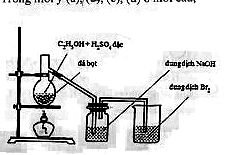
\includegraphics[width=0.48\textwidth]{images_gk2_hoa11_giahoi_2608/thi_nghiem_dieu_che_ethylene.png}
\end{center}
\choiceTF
{\True Vai trò của đá bọt là làm chất lỏng sôi đều và không bị trào ra.}
{Có thể thay dung dịch $\ce{H2SO4}$ đặc bằng dung dịch $\ce{H2SO4}$ 10\% vẫn thu được ethylene.}
{\True Khi ethylene sinh ra sẽ làm nhạt màu ống nghiệm đựng dung dịch $\ce{Br2}$, phản ứng xảy ra là phản ứng oxi hóa khử.}
{\True Trong phòng thí nghiệm, để thu khí ethylene, người ta dùng phương pháp đẩy nước.}

\loigiai{
a) \textbf{Đúng}: Đá bọt (chứa các mao quản xốp) đóng vai trò điều hòa quá trình sôi, phân tán nhiệt đều giúp chất lỏng sôi êm và tránh hiện tượng quá sôi cục bộ làm trào chất lỏng ra ngoài.\\
b) \textbf{Sai}: $\ce{H2SO4}$ đặc đóng vai trò vừa là chất xúc tác vừa là chất hút nước mạnh ở nhiệt độ cao ($\sim 170^\circ\text{C}$) để thực hiện phản ứng tách nước alcohol thành alkene. Dung dịch $\ce{H2SO4}$ loãng 10\% không có khả năng hút nước nên không thể tách nước tạo ethylene.\\
c) \textbf{Đúng}: Khí ethylene sinh ra phản ứng cộng với bromine làm nhạt màu/mất màu nước bromine:\\
$\ce{CH2=CH2 + Br2 -> CH2Br-CH2Br}$.\\
Trong phản ứng này, số oxi hóa của $\ce{C}$ tăng từ $-2$ lên $-1$ (chất khử), của $\ce{Br}$ giảm từ 0 xuống $-1$ (chất oxi hóa) $\implies$ đây là phản ứng oxi hóa -- khử.\\
d) \textbf{Đúng}: Do khí ethylene rất ít tan trong nước và nhẹ hơn không khí nên phương pháp tốt nhất để thu khí sạch trong phòng thí nghiệm là phương pháp đẩy nước.
}
\end{ex}
\begin{ex}
Benzene, toluene và styrene đều thuộc hợp chất hydrocarbon thơm (Arene).
\choiceTF
{Benzene, toluene và styrene đều có công thức chung là $\ce{C_n H_{2n-6}}$ ($n \ge 6$).}
{Styrene còn có tên gọi khác là ethylbenzene.}
{\True Để phân biệt benzene, toluene và styrene có thể dùng dung dịch $\ce{KMnO4}$.}
{So với benzene thì toluene phản ứng thế nguyên tử hydrogen ở vòng benzene dễ dàng hơn so với benzene và sản phẩm chính ưu tiên thế vào vị trí meta (\textit{-m}).}

\loigiai{
a) \textbf{Sai}: Benzene ($\ce{C6H6}$) và toluene ($\ce{C7H8}$) thuộc dãy đồng đẳng alkylbenzene có công thức chung $\ce{C_n H_{2n-6}}$ ($n \ge 6$). Styrene có công thức $\ce{C8H8}$ (có 1 vòng benzene và 1 nối đôi ở nhánh, độ bất bão hòa $k = 5$) nên có công thức tổng quát là $\ce{C_n H_{2n-8}}$.\\
b) \textbf{Sai}: Styrene là vinylbenzene ($\ce{C6H5-CH=CH2}$), còn ethylbenzene là hợp chất no ở mạch nhánh ($\ce{C6H5-CH2CH3}$).\\
c) \textbf{Đúng}: Sử dụng dung dịch $\ce{KMnO4}$:\\
- Styrene chứa liên kết đôi ở mạch nhánh nên làm mất màu dung dịch $\ce{KMnO4}$ ngay ở nhiệt độ thường.\\
- Toluene chỉ làm mất màu dung dịch $\ce{KMnO4}$ khi đun nóng.\\
- Benzene không làm mất màu dung dịch $\ce{KMnO4}$ kể cả khi đun nóng.\\
d) \textbf{Sai}: Nhóm methyl ($\ce{-CH3}$) là nhóm đẩy electron, làm tăng mật độ electron trong vòng thơm (đặc biệt tại các vị trí ortho và para), do đó phản ứng thế electrophile vào nhân thơm của toluene xảy ra dễ dàng hơn benzene và ưu tiên thế vào các vị trí ortho (\textit{-o}) và para (\textit{-p}), không phải meta (\textit{-m}).
}
\end{ex}
\vspace{4pt}
\noindent
{\color{mainGreen}\textbf{\large III. TRẮC NGHIỆM TRẢ LỜI NGẮN: (4 câu -- 2,0 điểm)}}\\
\textit{\small (Thí sinh ghi đáp án ngắn gọn vào ô/dòng trả lời)}
\vspace{2pt}

\begin{ex}
Trong số các hydrocarbon mạch hở sau: $\ce{C2H2, C4H10, C4H6, C4H8, C3H4, C3H6}$. Có bao nhiêu hydrocarbon có thể tạo kết tủa với dung dịch $\ce{AgNO3/NH3}$?

\loigiai{
Hydrocarbon mạch hở tác dụng với dung dịch $\ce{AgNO3/NH3}$ tạo kết tủa vàng là các alk-1-yne (có liên kết ba đầu mạch $\ce{-C#CH}$):\\
- $\ce{C2H2}$: ethyne ($\ce{CH#CH}$) $\implies$ có phản ứng.\\
- $\ce{C4H10}$: alkane no $\implies$ không phản ứng.\\
- $\ce{C4H6}$: mạch hở có đồng phân but-1-yne ($\ce{CH#C-CH2CH3}$) $\implies$ có thể tạo kết tủa.\\
- $\ce{C4H8}$: alkene/cycloalkane $\implies$ không phản ứng.\\
- $\ce{C3H4}$: propyne ($\ce{CH#C-CH3}$) $\implies$ có phản ứng.\\
- $\ce{C3H6}$: propene $\implies$ không phản ứng.\\
Vậy có 3 hydrocarbon thỏa mãn: $\ce{C2H2, C4H6, C3H4}$.\\
\textbf{Đáp số: 3}
}
\end{ex}
\begin{ex}
Phần trăm khối lượng của carbon (\%C) có trong phân tử ethylbenzene là bao nhiêu? \textit{(làm tròn đến hàng phần mười)}.

\loigiai{
Ethylbenzene có công thức phân tử là $\ce{C8H10}$ ($\ce{C6H5-C2H5}$).\\
Khối lượng mol: $M = 8 \times 12 + 10 \times 1 = 96 + 10 = 106\text{ g/mol}$.\\
Phần trăm khối lượng của carbon trong phân tử:\\
$\%C = \frac{96}{106} \times 100\% \approx 90{,}566\% \implies$ làm tròn đến hàng phần mười là \textbf{90,6\%}.\\
\textbf{Đáp số: 90,6\%}
}
\end{ex}
\begin{ex}
Trong các chất: $\ce{CH3Cl; CH3NH2; CH4O; CH2Br2; C2H4Cl2, HCl, C6H5F}$ có bao nhiêu chất thuộc loại dẫn xuất halogen của hydrocarbon?

\loigiai{
Dẫn xuất halogen của hydrocarbon được tạo thành khi thay thế một hay nhiều nguyên tử hydrogen trong phân tử hydrocarbon bằng một hay nhiều nguyên tử halogen ($\ce{F, Cl, Br, I}$).\\
- $\ce{CH3Cl}$ (chloromethane): dẫn xuất halogen.\\
- $\ce{CH3NH2}$ (methanamine): amine (chứa $\ce{N}$), không phải dẫn xuất halogen.\\
- $\ce{CH4O}$ (methanol): alcohol (chứa $\ce{O}$), không phải dẫn xuất halogen.\\
- $\ce{CH2Br2}$ (dibromomethane): dẫn xuất halogen.\\
- $\ce{C2H4Cl2}$ (dichloroethane): dẫn xuất halogen.\\
- $\ce{HCl}$ (hydrogen chloride): hợp chất vô cơ, không phải dẫn xuất của hydrocarbon.\\
- $\ce{C6H5F}$ (fluorobenzene): dẫn xuất halogen.\\
Vậy có 4 chất thuộc loại dẫn xuất halogen của hydrocarbon: $\ce{CH3Cl, CH2Br2, C2H4Cl2, C6H5F}$.\\
\textbf{Đáp số: 4}
}
\end{ex}
\begin{ex}
Da nhân tạo (PVC) được điều chế từ khí thiên nhiên theo sơ đồ:
$$\ce{CH4 -> C2H2 -> CH2=CH-Cl -> (-CH2-CHCl-)_n}$$
Nếu hiệu suất của toàn bộ quá trình điều chế là 20\%, muốn điều chế được 1,0 tấn PVC thì thể tích ($\text{m}^3$) khí thiên nhiên (chứa 80\% methane) ở điều kiện chuẩn cần dùng là bao nhiêu? \textit{(làm tròn kết quả đến hàng đơn vị)}.

\loigiai{
Khối lượng PVC cần sản xuất: $m_{\text{PVC}} = 1{,}0\text{ tấn} = 1000\text{ kg} = 10^6\text{ g}$.\\
Khối lượng mol của 1 mắt xích PVC ($\ce{-CH2-CHCl-}$) là: $M = 2 \times 12 + 3 \times 1 + 35{,}5 = 62{,}5\text{ g/mol}$.\\
Số mol mắt xích PVC cần tạo thành:\\
$n_{\text{PVC}} = \frac{10^6}{62{,}5} = 16\ 000\text{ mol} = 16\text{ kmol}$.\\
Theo sơ đồ bảo toàn nguyên tố carbon: $2\,\ce{CH4 -> 1}\text{ mắt xích PVC}$.\\
Số mol $\ce{CH4}$ lí thuyết cần dùng: $n_{\ce{CH4 (LT)}} = 2 \times n_{\text{PVC}} = 2 \times 16 = 32\text{ kmol}$.\\
Vì hiệu suất của toàn bộ quá trình là 20\% ($H = 0{,}2$) nên số mol $\ce{CH4}$ thực tế cần dùng là:\\
$n_{\ce{CH4 (TT)}} = \frac{32}{0{,}2} = 160\text{ kmol} = 160\ 000\text{ mol}$.\\
Khí thiên nhiên chứa 80\% methane theo thể tích (tương ứng 80\% theo số mol) nên số mol khí thiên nhiên cần dùng là:\\
$n_{\text{khí TN}} = \frac{160}{0{,}8} = 200\text{ kmol} = 200\ 000\text{ mol}$.\\
Ở điều kiện chuẩn ($25^\circ\text{C}, 1\text{ bar}$), thể tích khí thiên nhiên cần dùng là:\\
$V_{\text{khí TN}} = 200 \times 24{,}79 = \mathbf{4958\text{ m}^3}$.\\
(Nếu tính theo điều kiện tiêu chuẩn cũ $22{,}4\text{ L/mol}$: $V = 200 \times 22{,}4 = 4480\text{ m}^3$).\\
\textbf{Đáp số: 4958}
}
\end{ex}
\vspace{6pt}
\noindent
{\color{mainGreen}\textbf{\large IV. BÀI TẬP TỰ LUẬN: (3 câu -- 3,0 điểm)}}\\
\textit{\small (Học sinh trình bày chi tiết lời giải vào bài làm)}
\vspace{2pt}

\noindent
\textbf{Câu 1: (1,0 điểm)} Khí hóa lỏng hay khí gas (LPG -- Liquefied Petroleum Gas) được sử dụng làm nhiên liệu trong các hộ gia đình là propane hóa lỏng. Một bình khí gas hóa lỏng chứa 12,0 kg propane có thể cung cấp bao nhiêu Lít khí propane ở điều kiện chuẩn ($25^\circ\text{C}, 1\text{ bar}$)?

\begin{tcolorbox}[colback=white,colframe=solBlue,title=\textbf{Lời giải chi tiết và Biểu điểm Câu 1:}]
\begin{itemize}[leftmargin=1.2cm]
\item Khối lượng propane trong bình gas: $m = 12{,}0\text{ kg} = 12\ 000\text{ gam}$. \hfill \textit{(0,2 đ)}
\item Khối lượng mol của propane ($\ce{C3H8}$): $M = 3 \times 12 + 8 \times 1 = 44\text{ g/mol}$. \hfill \textit{(0,2 đ)}
\item Số mol propane chứa trong bình:
  $$n_{\ce{C3H8}} = \frac{12\ 000}{44} \approx 272{,}727\text{ mol}\quad \left(\text{hoặc } \frac{3000}{11}\text{ mol}\right). \hfill \textit{(0,3 đ)}$$
\item Ở điều kiện chuẩn ($25^\circ\text{C}, 1\text{ bar}$), 1 mol khí chiếm thể tích là $24{,}79\text{ Lít}$.\\
  Thể tích khí propane ở điều kiện chuẩn mà bình gas có thể cung cấp là:
  $$V = n \times 24{,}79 = \frac{3000}{11} \times 24{,}79 \approx \mathbf{6760{,}91\text{ Lít}}. \hfill \textit{(0,3 đ)}$$
  \textit{(Lưu ý: Nếu tính theo điều kiện tiêu chuẩn cũ $22{,}4\text{ L/mol}$: $V \approx 6109{,}09\text{ Lít}$)}.
\end{itemize}
\end{tcolorbox}

\vspace{4pt}
\noindent
\textbf{Câu 2: (1,0 điểm)} Nhựa PE (Polyethylene) là loại nhựa nhiệt dẻo phổ biến nhất thế giới, nổi bật với đặc tính dẻo dai, chống thấm nước, cách điện tốt và độ bền cao. Một trong những cách điều chế PE là theo sơ đồ: $\ce{C2H2 -> C2H4 -> polyethylene (PE)}$.\\
Viết các phương trình phản ứng thực hiện sơ đồ trên (ghi rõ điều kiện phản ứng).

\begin{tcolorbox}[colback=white,colframe=solBlue,title=\textbf{Lời giải chi tiết và Biểu điểm Câu 2:}]
\begin{itemize}[leftmargin=1.2cm]
\item (1) Phản ứng hydrogen hóa có chọn lọc chuyển acetylene thành ethylene:
  $$\ce{CH#CH + H2 ->[Pd/PbCO3, t^o] CH2=CH2} \hfill \textit{(0,5 đ)}$$
\item (2) Phản ứng trùng hợp ethylene điều chế polyethylene (PE):
  $$n\,\ce{CH2=CH2 ->[t^o, p, xt] (-CH2-CH2-)_n} \hfill \textit{(0,5 đ)}$$
\end{itemize}
\end{tcolorbox}

\vspace{4pt}
\noindent
\textbf{Câu 3: (1,0 điểm)} Thuốc nổ TNT (2,4,6-trinitrotoluene) được điều chế bằng phản ứng của toluene với hỗn hợp gồm $\ce{HNO3}$ đặc và $\ce{H2SO4}$ đặc, trong điều kiện đun nóng. Biết hiệu suất của toàn bộ quá trình tổng hợp là 60\%. Lượng TNT (2,4,6-trinitrotoluene) tạo thành từ 552,0 gam toluene là bao nhiêu gam?

\begin{tcolorbox}[colback=white,colframe=solBlue,title=\textbf{Lời giải chi tiết và Biểu điểm Câu 3:}]
\begin{itemize}[leftmargin=1.2cm]
\item Phương trình hóa học điều chế 2,4,6-trinitrotoluene (TNT):
  $$\ce{C6H5CH3 + 3HNO3 ->[H2SO4 đ, t^o] C6H2(NO2)3CH3 + 3H2O} \hfill \textit{(0,25 đ)}$$
  \textit{(Khối lượng mol: Toluene $M = 92\text{ g/mol}$; TNT $M = 227\text{ g/mol}$)}.
\item Số mol toluene ban đầu:
  $$n_{\text{toluene}} = \frac{552{,}0}{92} = 6{,}0\text{ mol}. \hfill \textit{(0,25 đ)}$$
\item Theo phương trình phản ứng, số mol TNT lí thuyết thu được:
  $$n_{\text{TNT (LT)}} = n_{\text{toluene}} = 6{,}0\text{ mol}. \hfill \textit{(0,2 đ)}$$
\item Do hiệu suất của toàn bộ quá trình là 60\% nên số mol TNT thực tế thu được là:
  $$n_{\text{TNT (TT)}} = 6{,}0 \times 60\% = 3{,}6\text{ mol}. \hfill \textit{(0,15 đ)}$$
\item Khối lượng TNT (2,4,6-trinitrotoluene) tạo thành:
  $$m_{\text{TNT}} = 3{,}6 \times 227 = \mathbf{817{,}2\text{ gam}}. \hfill \textit{(0,15 đ)}$$
\end{itemize}
\end{tcolorbox}

\vspace{8pt}
\begin{center}
\textbf{--------- HẾT ---------}
\end{center}

\end{document}
